\documentclass{article}
\usepackage{tikz}
\usepackage{natbib}
\title{Introduction to Stan: problem set}
\date{}
\usepackage{caption}
\captionsetup{font=footnotesize}
\usepackage[utf8]{inputenc}
\usepackage{amsmath}
\usepackage{multimedia}
\usepackage{animate}
\usepackage{graphics}
\usepackage{graphicx}
\usepackage[makeroom]{cancel}
\newtheorem{problem}{Problem}[section]
\usepackage{bbm}
\author{Ben Lambert}
\usepackage{listings}
\usepackage{minted}

\begin{document}
\maketitle

\section{Stan entry level: discoveries data}
The file ``discoveries.csv" contains data on the numbers of ``great'' inventions and scientific discoveries ($X_t$) in each year from 1860 to 1959 \citep{discoveries}. In this question you will develop a model to explain the variation in scientific inventions across time. The simplest model here is to assume that \textbf{a.} one discovery occurs independently of all others, and \textbf{b.} the rate of occurrence of discoveries is the same in all years. Since the data is discrete, these assumptions suggests use of a Poisson model:

\begin{equation}
X_t\sim \text{Poisson}(\lambda)
\end{equation}

\begin{problem}
Open an editor and create a file called ``discoveries.stan'' in your working directory. In the file create three parameter blocks:
	
\begin{minted}{stan}
data {
	
}
parameters {
	
}
model {
	
}
\end{minted}	
\end{problem}

\begin{problem}
Fill in the data and parameter blocks for the above model.
\end{problem}

The completed model can be written as:
\begin{minted}{stan}
data {
    int N; ## number of observations
    int<lower=0> X[N]; ## vector of discoveries
}
parameters {
    real<lower=0> lambda;
} 
model {
     X ~ poisson(lambda); ## likelihood
    lambda ~ lognormal(2,1); ## prior
}
\end{minted}	


\begin{problem}
	Using a log-normal(2,1)  prior for $\lambda$ code up the ``model'' block, making sure to save your file afterwards.
\end{problem}

\begin{problem}
	Open your statistical software (R, python, matlab, etc.) and load any packages necessary to use Stan. (Hint: in R this is done by using ``library(rstan)'; in Python this is done using ``import pystan''.)
\end{problem}

\begin{problem}
Load the ``discoveries.csv" data and graph the data. What does this suggest about our model's assumptions?
\end{problem}

Both a time series and histogram are useful here (see figure \ref{fig:discoveriesTime}). To me the left hand plot suggests that there is some temporal autocorrelation in the data (perhaps invalidating an assumption of independence, and/or identical distribution). The histogram would seem to support this claim, since the variance is fairly obviously greater than the mean. I also plot an autocorrelogram of the data which suggests that there is autocorrelation in the series.

\begin{figure}[ht]
	\centerline{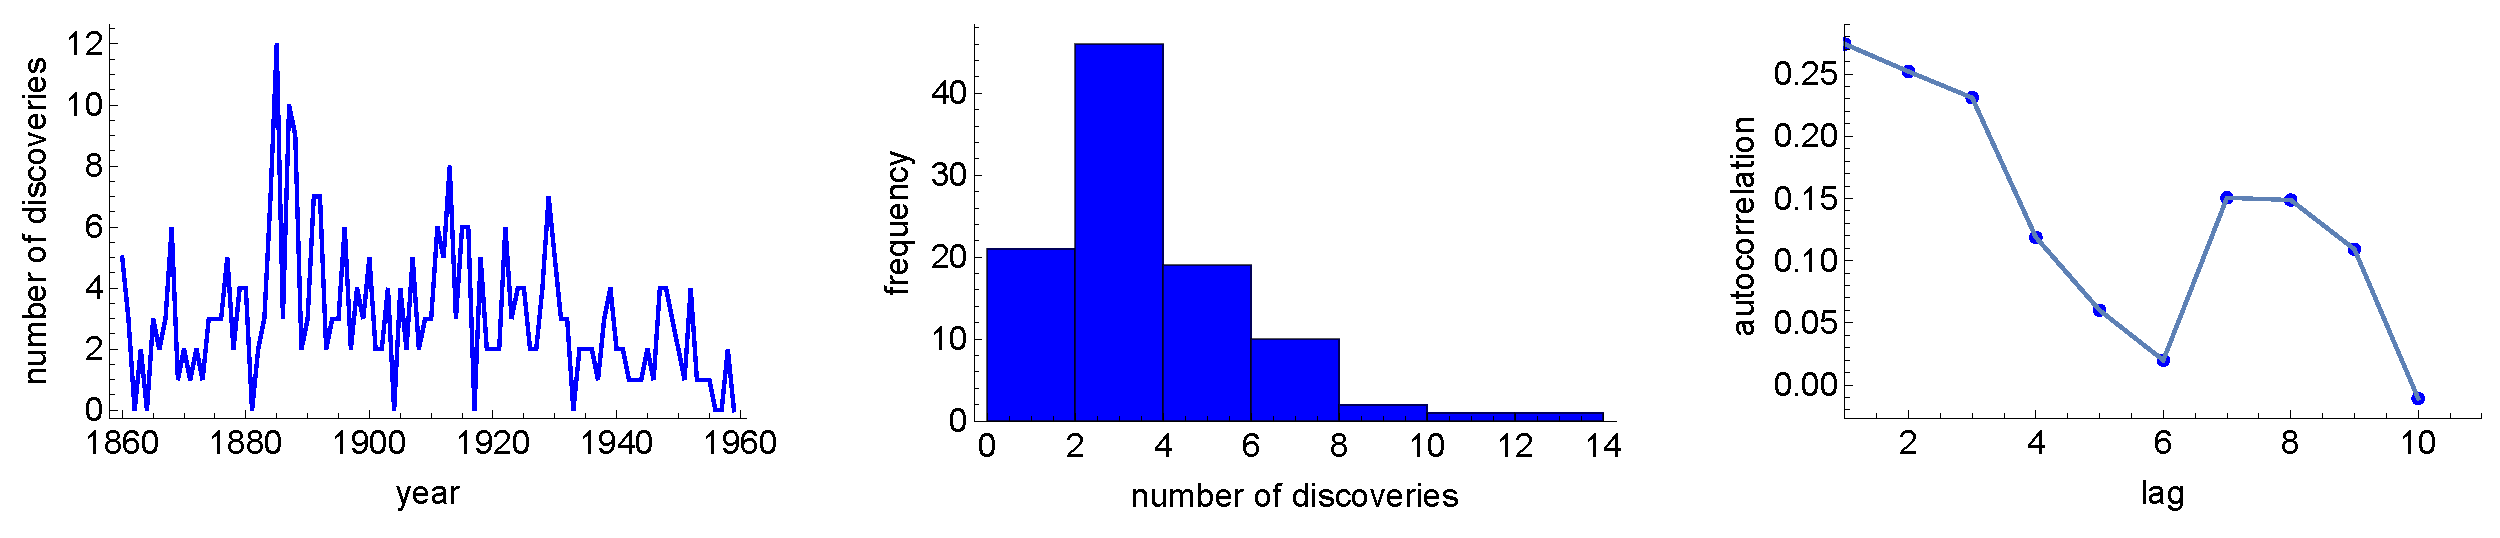
\includegraphics[width=1.5\textwidth]{figures/prob2_discoveriesTime.pdf}}
	\caption{Characteristics of the ``discoveries'' data set.}\label{fig:discoveriesTime}
\end{figure}

\begin{problem}
Load the data into your software then put it into a structure that can be passed to Stan. (Hint: in R create a list of the data; in Python create a dictionary where the `key' for each variable is the desired variable name.)

\begin{minted}{R}
aDF <- read.csv('discoveries.csv')
X <- aDF[,2]
N <- length(X)
dataList <- list(N=N,X=X)
\end{minted}
\end{problem}

\begin{problem}
Fit your model using Stan, with 4 chains, each with a sample size of 1000, and a warm-up of 500 samples. Set seed=1 to allow reproducibility of your results. Store your result in an object called ``fit''.
\end{problem}

\begin{minted}{R}
fit <- stan(file = 'discoveries.stan',data=dataList,
            iter=1000,chains=4,seed=1)
\end{minted}

\begin{problem}
Diagnose whether your model has converged by printing ``fit''.
\end{problem}

Lambda and lp should both have a value of $\hat{R}\approx 1$.

\begin{problem}
For your sample what is the equivalent number of samples for an independent sampler?
\end{problem}

This is just the value of ``n\_eff'' which I get to be around 600-900.

\begin{problem}
Find the central posterior 80\% credible interval for $\lambda$.
\end{problem}

This can be done in R by the following:

\begin{minted}{R}
print(fit,pars = 'lambda',probs = c(0.1,0.9))
\end{minted}

Alternatively, you can extract lambda from the fit object then find its quantiles:

\begin{minted}{R}
lLambda <- extract(fit,'lambda')[[1]]
c(quantile(lLambda,0.1),quantile(lLambda,0.9))
\end{minted}

Or in Python by doing:

\begin{minted}{python}
import numpy as np
lambda_samples = fit.extract('lambda')['lambda']
np.percentile(lambda_samples, (10, 90))
\end{minted}

In any case I get an interval of approximately $2.9\leq\lambda\leq 3.3$.

\begin{problem}
	Draw a histogram of your posterior sample for $\lambda$.
\end{problem}

To do this in R, first extract the parameter, then draw the plot.

\begin{minted}{R}
library(ggplot2)

lLambda <- extract(fit,'lambda')[[1]]
qplot(lLambda)
\end{minted}

Or in Python:

\begin{minted}{python}
import numpy as np
import matplotlib.pyplot as plt
lambda_samples = fit.extract('lambda')['lambda']
np.percentile(lambda_samples, (10, 90))
plt.hist(lambda_samples)
plt.xlabel("lambda")
plt.ylabel("frequency")
\end{minted}

\begin{problem}
	Create a ``generated quantities'' block in your Stan file, and use it to sample from the posterior predictive distribution (Hint: use the function ``poisson\_rng'' to generate independent samples from your lambda).
\end{problem}

\begin{minted}{stan}
generated quantities{
    int<lower=0> XSim[N];
    for (i in 1:N){
        XSim[i] <- poisson_rng(lambda);
    }
}
\end{minted}

\begin{problem}
	Carry out appropriate posterior predictive checks to evaluate your model.
\end{problem}

One simple check is to compare the maximum of your posterior predictive simulations with that of the real data (which is 12 discoveries in 1885.) To do this in R do something like the following:

\begin{minted}{R}
lXSim <- extract(fit,'XSim')[[1]]
lMax <- apply(lXSim, 1,max)

library(ggplot2)
qplot(lMax)

mean(lMax>=12)
\end{minted}

Or in Python by:

\begin{minted}{python}
posterior_checks = fit.extract('XSim')['XSim']
posterior_checks_max = np.amax(posterior_checks, axis=1)
(posterior_checks_max >= 12).sum() / float(len(posterior_checks_max))
\end{minted}

From the resultant histogram it is evident that our model would only very rarely produce 12 discoveries. I get 12+ discoveries in only about 1\% of simulations. 

\begin{problem}
	A more robust sampling distribution is a negative binomial model:
	
	\begin{equation}
	X_i \sim \text{negative-binomial}(\mu,\kappa)
	\end{equation}
	
	where $\mu$ is the mean number of discoveries per year, and $var(X) = \mu + \frac{\mu^2}{\kappa}$. Here $\kappa$ measures the degree of over-dispersion of your model; specifically if $\kappa\uparrow$ then over-dispersion$\downarrow$.  
	
	Write a new stan file called ``discoveries\_negbin.stan'' that uses this new sampling model (Hint: use the Stan manual section on discrete distributions to search for the correct negative binomial function name; be careful there are two different parameterisations of this function available in Stan!) Assume that we are using the following priors:

\begin{align}
\mu&\sim \text{log-normal}(2,1)\\
\kappa&\sim \text{log-normal}(2,1)\\
\end{align}
	
	Draw 1000 samples across 4 chains for your new model. Has it converged to the posterior? 
\end{problem}

The full code should be something like:

\begin{minted}{stan}
data {
    int N;
    int<lower=0> X[N];
}
parameters {
    real<lower=0> mu;
    real<lower=0> kappa;
} 
model {
    X ~ neg_binomial_2(mu,kappa);
    mu ~ lognormal(2,1);
    kappa ~ lognormal(2,1);
}
\end{minted}	

After 1000 samples across 4 chains I get a value of $\hat{R}\approx 1$, and an effective sample size around 1000. 

\begin{problem}
	Carry out posterior predictive checks on the new model. What do you conclude about the use of a negative binomial here versus the simpler Poisson?
\end{problem}

The Stan code to generate the posterior predictive distribution samples is:

\begin{minted}{stan}
generated quantities{
    int<lower=0> XSim[N];
    for (i in 1:N){
        XSim[i] <- neg_binomial_2_rng(mu,kappa);
    }
}
\end{minted}

Now I obtain about 20\% of posterior predictive samples that have a maximum value greater than or equal to 12 (that of the real data). This is much more reasonable than that from the Poisson model.

\begin{problem}
	Find the central posterior 80\% credible interval for the new mean rate of discoveries $\mu$. How does it compare with your results from the Poisson model? Why is this the case?
\end{problem}

I get a similar answer to before, around: $2.8\leq\lambda\leq 3.4$; it should be slightly wider because there is more sampling variability $\implies$ greater uncertainty over the parameter's value.

\begin{problem}
	(Optional) Calculate the autocorrelation in the residuals between the actual and simulated data series. What do these suggest about our current model?
\end{problem}

If you look at the autocorrelation you see that there is a slight, yet persistent, positive autocorrelation (looking at the first lag). You can obtain these in R by the following:

\begin{minted}{R}
lXSim <- extract(fit,'XSim')[[1]]
mResid <- sweep(lXSim,2,X)
lCorr <- sapply(seq(1,200,1),function(i) acf(mResid[i,],lag.max = 1)$acf[[2]])
qplot(lCorr)
\end{minted}

\begin{problem}
	Optional: following on from the above suggest an alternative model formulation.
\end{problem}

Clearly there is some persistence in the rate of discoveries over time. In other words, discoveries tend to clump together. This is clear from a simple time series plot of the data. One idea would be to allow an AR1 process for the mean of the process:

\begin{equation}
\mu(t) = \rho \mu(t-1) + (1-\rho) \bar{\mu} + \epsilon(t)
\end{equation}

This allows for persistence in the rate over time.


\section{Stan entry level : Hungover holiday regressions}
The data in file ``hangover.csv'' contains a series of Google Trends estimates of the search traffic volume for the term ``hangover cure'' in the UK between February 2012 to January 2016. The idea behind this problem is to determine how much more hungover are people in the ``holiday season'' period, defined here as the period between 10th December and 7th January, than the average for the rest of the year.

\begin{problem}
	Graph the search volume over time, and try to observe the uplift in search volume around the holiday season.
\end{problem}

\begin{minted}{R}
plot(as.Date(hangover$date),hangover$volume,type='l',xlab = 'date',ylab = 'volume')
\end{minted}

Shows obvious spikes during the holiday season period.

\begin{problem}
The variable ``holiday'' is a type of indicator variable that takes the value 1 if the given week is \textit{all} holiday season, 0 if it contains none of it, and $0<X<1$ for a week that contains a fraction $X$ of days that fall in the holiday season. Graph this variable over time so that you understand how it works.
\end{problem}

\begin{problem}
A simple linear regression is proposed of the form,

\begin{equation}
V_t\sim \text{normal}(\beta_0+\beta_1 h_t,\sigma)
\end{equation}

where $V_t$ is the search volume in week $t$ and $h_t$ is the holiday season indicator variable. Interpret $\beta_0$ and $\beta_1$ and explain how these can be used to estimate the increased percentage of hangovers in the holiday season.
\end{problem}

$\beta_0$ is the average hangover search volume in weeks that aren't in the holiday season, and $\beta_1$ shows the uplift for a week that falls in the holiday season. The percentage increase is hence $\beta_1/\beta_0$.

\begin{problem}
	Assuming $\beta_i\sim N(0,50)$ and $\sigma\sim \text{half-normal}(0,10)$ priors write a Stan model to estimate the percentage increase in hangoverness over the holiday period.
\end{problem}

An example stan program is shown below (not the most efficient since doesn't vectorise, but the below is simplest to understand),

\begin{minted}{Stan}
data{
  int T;
  real V[T];
  real h[T];
}

parameters{
  real beta0;
  real beta1;
  real<lower=0> sigma;
}

model{
  for(t in 1:T)
    V[t] ~ normal(beta0 + beta1 *h[t],sigma);
  beta0 ~ normal(0,50);
  beta1 ~ normal(0,50);
  sigma ~ normal(0,10);
}

generated quantities{
  real uplift;
  uplift = beta1 / beta0;
}
\end{minted}

From this I estimate that with 50\% probability $77\% \leq \text{uplift} \leq 86\%$!

\section{Stan middle level: coding up a bespoke probability density}
In the file ``survival.csv'' there are data for a variable $Y$ that we believe comes from a probability distribution $p(Y) =\frac{\sqrt[3]{b}}{\Gamma\left(\frac{4}{3}\right)} exp(-b Y^3)$ where $b>0$ is a parameter of interest. In this question we are going to write a Stan program to estimate the parameter $b$ even though this distribution is not amongst Stan's implemented distributions.

\begin{problem}
	Explain what is meant by the following statement in Stan,
	
	\begin{minted}{Stan}
	theta ~ beta(1,1);
	\end{minted}
	
	In particular, explain why this is equivalent to the following,
	
	\begin{minted}{Stan}
	target += beta_lpf(theta|1,1);
	\end{minted}
	
	where \mintinline{Stan}{target} is a Stan variable that stores the overall log-probability, and \mintinline{Stan}{+=} increments \mintinline{Stan}{target} by an amount corresponding to the RHS.
	
\end{problem}

\mintinline{Stan}{~} statements in Stan do not mean sampling! They always mean increment the log probability by something since HMC works in the (negative) log probability space. In this case it means increment the log probability by an amount corresponding to the probability density of a value ``theta'' from a beta(1,1) distribution. This is why it is equivalent to the second piece of code where we explicitly increment the log probability. 

Note there is a subtle difference between the two which is that \mintinline{Stan}{~} statements drop all constant terms from the log probability update, whereas the target statements keep these. However for most purposes this is not important.


\begin{problem}
	By hand work out an expression for the log-probability for a density $p(Y) =\frac{\sqrt[3]{b}}{\Gamma\left(\frac{4}{3}\right)} exp(-b Y^3)$.
\end{problem}

Just take the log of the expression,

\begin{align}
log\; p = log\left(\frac{\sqrt[3]{b}}{\Gamma(4/3)}\right) - b y^3
\end{align}

\begin{problem}
	Write a Stan function that for a given value of $y$ and $b$ calculates the log probability (ignoring any constant terms). Hint: Stan functions are declared as follows,
	
\begin{minted}{Stan}
functions{
  real anExample(real a, real b){
    ...
    return(something);
  }
}
\end{minted}
	
	where in this example the function takes two reals as inputs and outputs something of type real.
\end{problem}

A function to do this is shown below,

\begin{minted}{Stan}
functions{
  real fCustomProb(real aY, real aB){
    real aConst;
    aConst = (aB^(1.0/3.0));
    return(log(aConst) - aB * (aY^3));
  }
}
\end{minted}

\begin{problem}
Use your previously created function to write a Stan program that estimates $b$, and then use it to do so with the $y$ series contained within ``survival.csv''. Hint: Stan functions must be declared at the top of a Stan program.
\end{problem}

An example Stan file is given below,

\begin{minted}{Stan}
functions{
  real fCustomProb(real aY, real aB){
    real aConst;
    aConst = (aB^(1.0/3.0));
    return(log(aConst) - aB * (aY^3));
  }
}

data{
  int N;
  real Y[N];
}

parameters{
  real<lower=0> b;
}

model{
  for(i in 1:N)
    target += fCustomProb(Y[i],b);
}
\end{minted}

which when run estimates a posterior mean for $b$ $\approx$ 2.42.

\section{Stan advanced level: is a tumour benign or malignant?}
Suppose that if a tumour is benign the result of a clinical test for the disease for individual $i$ is $X_i\sim \text{binomial}(20,\theta_b)$, whereas if the tumour is malignant $X_i\sim \text{binomial}(20,\theta_m)$, where $\theta_b < \theta_m$. Suppose that we collect data on 10 patients' scores on this clinical test $X=\{4,18,6,4,5,6,4,6,16,7\}$ and would like to infer the disease status for each individual, as well as the parameters $(\theta_b,\theta_m)$.

\begin{problem}
	Write down in pseudo-code the full model, where we suppose that we use uniform priors on $(\theta_b,\theta_m)$ and discrete uniform priors on the disease status $s_i$ of individual $i$.
\end{problem}

This looks like,

\begin{align}
s_i &\sim \text{discrete-uniform}(1,2)\\
\text{if} \;\;\;&(s_i = 1)\\
X_i &\sim \text{binomial}(10,\theta_b)\\
\text{else} &\\
X_i &\sim \text{binomial}(10,\theta_m)
\end{align}

\begin{problem}
	Assuming that $s_i\in[1,2]$ is the disease status of each individual (1 corresponding to a benign growth, and 2 to a malignant one), use the \mintinline{Stan}{transformed parameters} block to calculate the log probability of each individual's data. Hint: this will be a 10 $\times$ 2 matrix, where the 2 corresponds to each possible disease status.
\end{problem}

\begin{minted}{stan}
transformed parameters{
  matrix[10,2] lp;
  for(i in 1:10){
    for(s in 1:2){
      lp[i,s] = log(0.5) + binomial_lpmf(X[i]|N,theta[s]);
    }
  }
}
\end{minted}

\begin{problem}
	The disease status of each individual $s_i\in[1,2]$ is a discrete variable, and because Stan does not support discrete parameters directly it is not as straightforward to code up these problems as for continuous parameter problems. The way that to do this is by marginalising out $s_i$ from the joint distribution,
	
	\begin{equation}
	p(\theta_b,\theta_m|X) = \sum_{s_1=1}^{2} p(\theta_b,\theta_m,s_1|X)
	\end{equation}
	where we have illustrated this for the disease status of individual 1. This then allows us to find an expression for the posterior density which we log to give $lp$, and then use \mintinline{Stan}{target+=lp} to increment the log probability. However, because we do this on the log density scale we instead do the following,
	
	\begin{align}
	\text{log} \; p(\theta_b,\theta_m|X) &= \text{log} \sum_{s_1=2}^{K} p(\theta_b,\theta_m,s_1|X)\\
	&= \text{log} \sum_{s_1=1}^{2} exp\left( log\; p(\theta_b,\theta_m,s_1|X)\right)\\
	&= \text{log}\_\text{sum}\_\text{exp}_{s_1=1}^{2}(\text{log}\; p(\theta_b,\theta_m,s_1|X))
	\end{align}
	
	where \mintinline{Stan}{log_sum_exp(.)} (a function available in Stan) is defined as,
	
	\begin{equation}
	\text{log\_sum\_exp}_{i=1}^{K} \alpha = log\; \sum_{i=1}^{K} exp(\alpha) 
	\end{equation}
	
	and is a more numerically-stable way of doing the above calculation. Using this knowledge, write a full Stan model that implements this marginalisation, and use it to estimate $\theta_b$ and $\theta_m$. Hint: use the \mintinline{Stan}{binomial_logit_lpmf(X[i]|N,alpha[s])} function in Stan and define \mintinline{Stan}{ordered[2] alpha}, then transform from the unconstrained alpha to theta using \mintinline{Stan}{inv_logit}.
\end{problem}

The below code is one such implementation of this model,

\begin{minted}{Stan}
data { 
  int<lower=1> nStudy; // num studies
  int<lower=1> N; // samples per study
  int<lower=0, upper=N> X[nStudy]; // number successes
} 

parameters { 
  ordered[2] alpha; 
}

transformed parameters{
  real<lower=0,upper=1> theta[2];
  matrix[nStudy,2] lp;
  for(i in 1:2){
    theta[i] = inv_logit(alpha[i]);
  }

  for(n in 1:nStudy){
    for(s in 1:2){
      lp[n,s] = log(0.5) + 
        binomial_logit_lpmf(X[n]|N,alpha[s]);
    }
  }
}

model { 
  for(n in 1:nStudy){
    target += log_sum_exp(lp[n]);
  }
}
\end{minted}

This should yield $\theta_b\approx 0.2-0.3$ and $\theta_m \approx 0.8-0.9$.

\begin{problem}
	We use the \mintinline{stan}{generated quantities} block to estimate the probabilities of state $s=1$ in each different experiment by averaging over all $L$ posterior draws,
	
	\begin{equation}
	q(s=1|X) \approx \frac{1}{L} \sum_{i=1}^{L} q(s=1,\text{alpha}[s=1]|X)
	\end{equation}
	
	where $q(.)$ is the un-normalised posterior density. The averaging over all posterior draws is necessary to marginalize out the alpha parameter. To normalise the posterior density we therefore divide the above by the sum of the un-normalised probability across both states,
	
	\begin{equation}
	Pr(s=1|X) = \frac{q(s=1|X)}{q(s=1|X)+q(s=2|X)}
	\end{equation} 
	
	Using the above knowledge add a \mintinline{stan}{generated quantities} block to your Stan model that does this, and hence estimate the probability that each individual's tumour is benign.
\end{problem}

\begin{minted}{Stan}
generated quantities{
  matrix[nStudy,2] pstate;
  for(n in 1:nStudy){
    pstate[n] = exp(lp[n]-log_sum_exp(lp[n]));
  }
}
\end{minted}

Apart from unlucky individuals 2 and 9 where $p(benign)\approx 0$ all other individuals' $p(benign)\approx 1$.


\section{Stan advanced level: how many times did I flip the coin?}
Suppose that I have a coin with $\theta$ denoting the probability of it landing heads-up. In each experiment, I flip the coin $N$ times, where $N$ is unknown to the observer and record the number of heads obtained $Y$. I repeat the experiment 10 times, each time flipping the coin the same $N$ times, and record $Y=\{9,7,11,10,10,9,8,11,9,11\}$ heads.

\begin{problem}
	Write down an expression for the likelihood, stating any assumptions you make.
\end{problem}

Assuming independent and identically-distributed observations we obtain,

\begin{align}
Y_i\sim \text{binomial}(N,\theta)
\end{align}

\begin{problem}
	Suppose that the maximum number of times the coin could be flipped is 20, and that all other (allowed) values we regard \textit{a priori} as equally probable. Further suppose that based on previous coin flipping experiences we specify a prior $\theta\sim \text{beta}(7,2)$. Write down the model as a whole (i.e. the likelihood and the priors).
\end{problem}

\begin{align}
Y_i &\sim \text{binomial}(N,\theta)\\
N &\sim \text{discrete-uniform}(11,20)\\
\theta &\sim \text{beta}(7,2)
\end{align}

\begin{problem}
	This problem can be coded in Stan by marginalising out the discrete parameter $N$. The key to doing this is writing down an expression for the log-probability for each result $Y_i$ conditional on an assumed value of $N$, and $\theta$. Explain why this can be written in Stan as,
	
	\begin{minted}{Stan}
	log(0.1) + binomial_lpmf(Y[i]|N[s],theta);  
	\end{minted}
	
	where \mintinline{stan}{N[s]} is the sth element of a vector $N$ containing all possible values for this variable.
	
\end{problem}


\begin{problem}
	In the \mintinline{stan}{transformed parameters} block write code that calculates the log probability for each experiment and each possible value of $N$.
\end{problem}

\begin{minted}{Stan}
transformed parameters{
  vector[10] lp;
  for(s in 1:10){
    lp[s] = log(0.1) + binomial_lpmf(Y|N[s],theta);  
  }
}
\end{minted}

The above uses the vectorised form of the RHS, which is important because it allows $N$ to be the same across all experiments (I fell foul of this when I initially coded it up!)

\begin{problem}
	Write a Stan program to estimate $\theta$. Hint: in the \mintinline{Stan}{model} block use \mintinline{Stan}{target+= log_sum_exp(lp)} to marginalise out $N$ and increment the log probability. 
\end{problem}

The Stan program is,

\begin{minted}{Stan}
data{
  int K;
  int Y[K];
}

transformed data{
  int N[10];
  for(s in 1:10){
    N[s] = 10 + s;
  }
}

parameters{
  real<lower=0,upper=1> theta;
}

transformed parameters{
  vector[10] lp;
  for(s in 1:10){
    lp[s] = log(0.1) + binomial_lpmf(Y|N[s],theta);  
  }
}

model{
  for(i in 1:K){
    target += log_sum_exp(lp[i]);
  }
  theta ~ beta(7,2);
}
\end{minted}

For a definition of \mintinline{Stan}{log_sum_exp(.)} see the answer to the next question. The posterior mean of $\theta$ is about 0.78, with a 95\% HDI of $0.54\leq \theta \leq 0.91$.

\begin{problem}
	Use the \mintinline{Stan}{generated quantities} block to estimate the probabilities of each state.
\end{problem}

This relies on us estimating the un-normalised density for the number of coin flips by averaging over all samples for $\theta$,

\begin{equation}
q(N=11|Y) \approx \frac{1}{L} \sum_{i=1}^{L} q(N=11,\theta_i|Y)
\end{equation}

where $q(.)$ is the un-normalised posterior density and $L$ is the number of posterior samples. To normalise this density we then divide the above by the un-normalised density for all other possible values for $N$,

\begin{equation}
Pr(N=11|Y) = \frac{q(N=11|Y)}{\sum_{N=11}^{20} q(N=i|Y)}
\end{equation}

To do this in Stan we use  \mintinline{Stan}{log_sum_exp(.)} which is defined as,

\begin{equation}
\text{log\_sum\_exp}_{i=1}^{K} \alpha = log\; \sum_{i=1}^{K} exp(\alpha) 
\end{equation}

which allows us to marginalise out any dependence on $N$ in log prob space because,

\begin{align}
\text{log} \; p(\theta) &= \text{log} \sum_{N=1}^{K} p(\theta,N)\\
&= \text{log} \sum_{N=1}^{K} exp\left( log\; p(\theta,N)\right)\\
&= \text{log}\_\text{sum}\_\text{exp}_{N=1}^{K}(\text{log}\; p(\theta,N))
\end{align}

So implementing this in Stan we have,

\begin{minted}{Stan}
generated quantities { 
  simplex[10] pState;
  pState = exp(lp - log_sum_exp(lp)); 
} 
\end{minted}

which results in probabilities of each state shown in figure \ref{fig:coinFlip_boxPlot}. Note that it is better to use the expectation once, rather than do exp(something) over exp(something else) because this risks numerical accuracy.

\begin{figure}[ht]
	\centerline{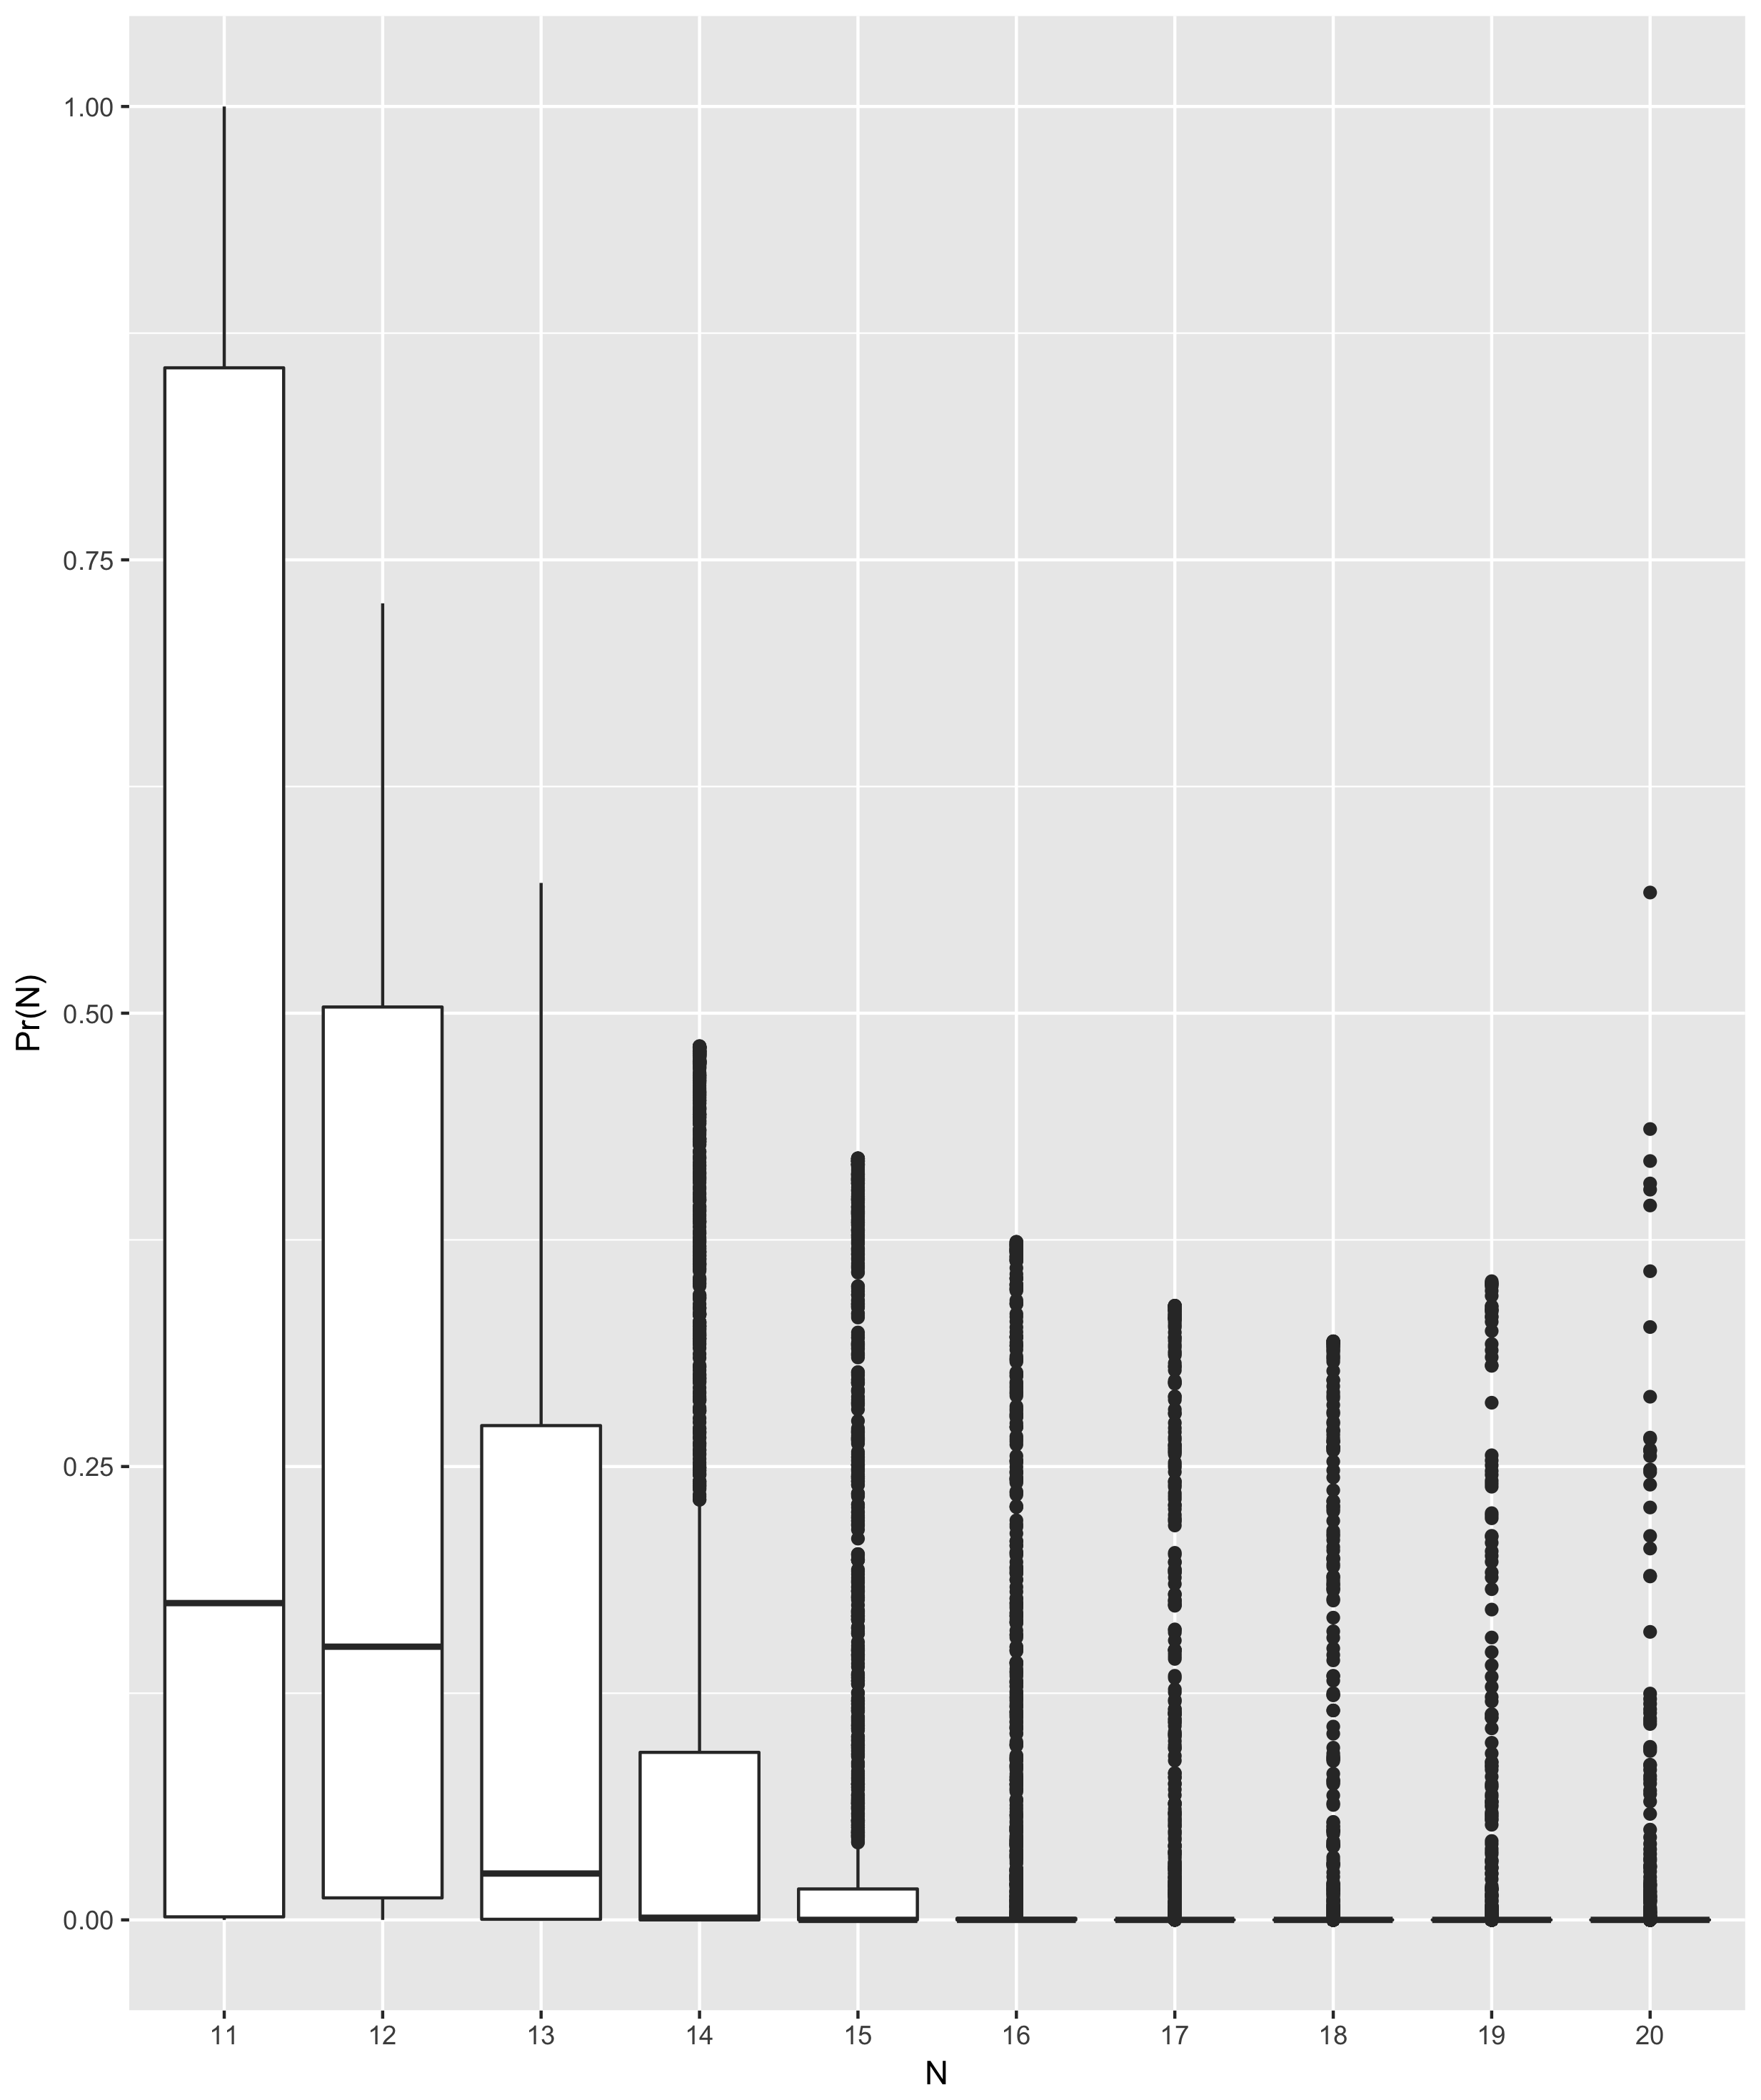
\includegraphics[width=1\textwidth]{figures/coinFlip_boxplot.png}}
	\caption{The estimated probabilities for each $N$ in the coin flipping example.}\label{fig:coinFlip_boxPlot}
\end{figure} 


\bibliographystyle{plain} 
\bibliography{bibliography}

\end{document}
